% Block diagram of the dispatcher, rendered to dispatcher.png by "make
% diagrams" (see the DIAGRAMS variable in the top-level Makefile). It is
% shown in ALGORITHM.md, in the section "Timing of a job and a result" of the
% Dispatcher, whose tables give the clock cycle of each step.
%
% This replaces an ASCII drawing in ALGORITHM.md. Anything that changes the
% processes or the registers of the dispatcher has to change this file too.
%
% What it shows: the two parts of the dispatcher (dispatcher_jobs.vhd and
% dispatcher_results.vhd) and the job modules between them, each part with its
% processes in the order a job or a result goes through them, and the
% registers each process writes. The arrows are the signals between the parts
% and to the outside. All of them come from registers, which is what lets
% ALGORITHM.md follow a job and a result one clock cycle at a time. The
% dotted box is the entity dispatcher (dispatcher.vhd).
%
% What it does not show: the groups of 16 job modules, which every process
% that ends in "in each group" has one register per group for; the reset; and
% the schedulers' own internals beyond the register named.

\documentclass[border=8pt]{standalone}

\usepackage[T1]{fontenc}
\usepackage{helvet}
\renewcommand{\familydefault}{\sfdefault}

\usepackage{array}
\usepackage{tikz}
\usetikzlibrary{arrows.meta, positioning, fit, calc}

% A process of a part, and what it registers: the process in typewriter, the
% registers as text, in a two-column table inside the block.
\newcommand{\proc}[2]{\texttt{#1} & #2 \\}

\begin{document}

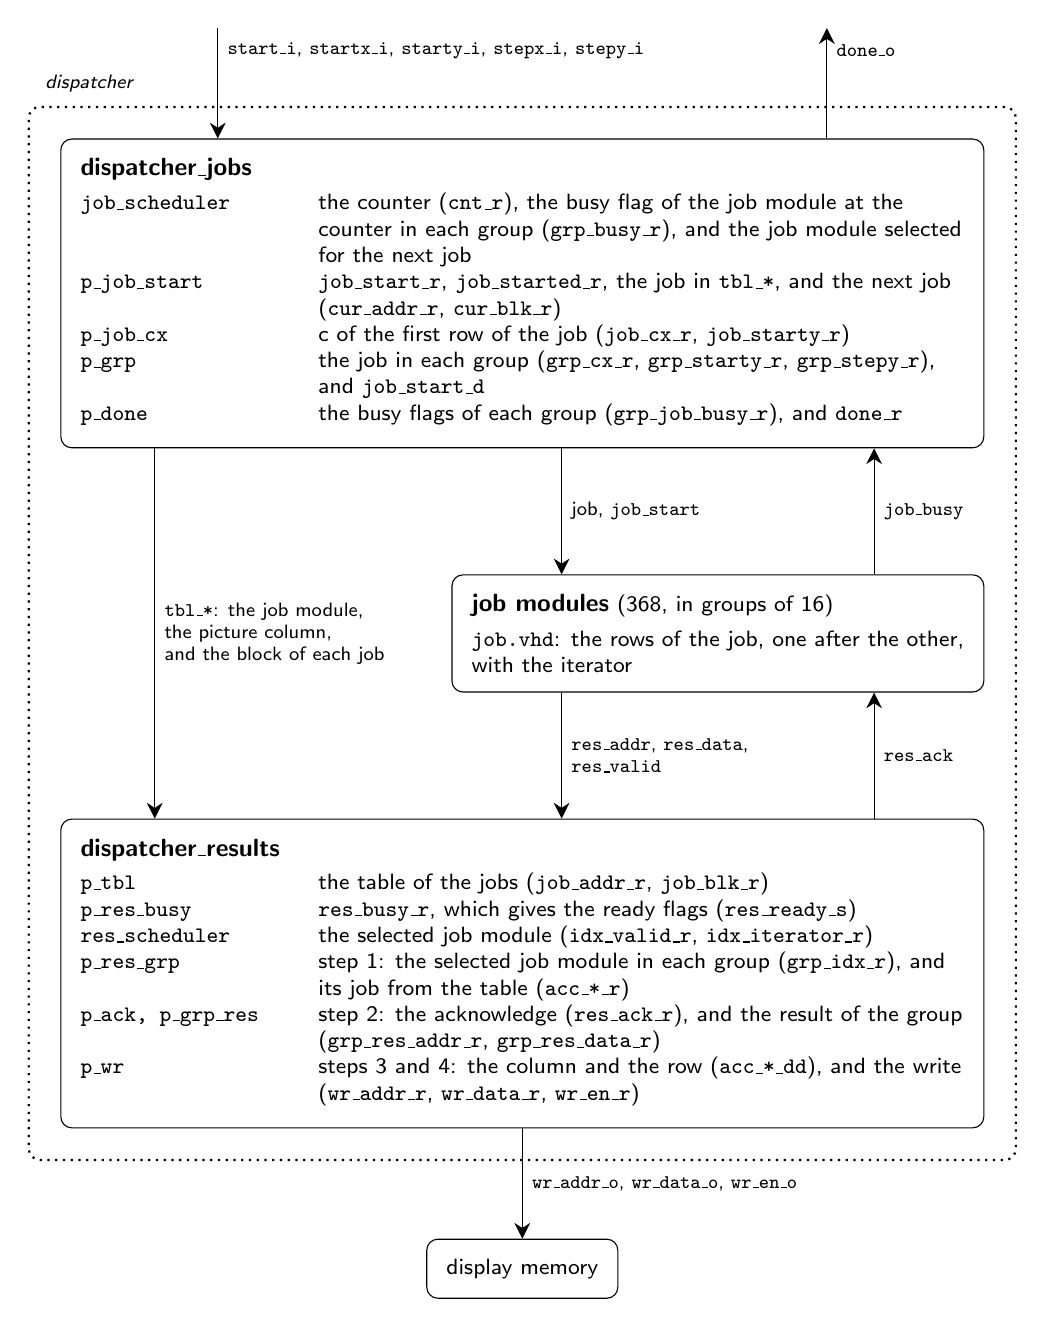
\begin{tikzpicture}[
      font = \sffamily\footnotesize,
      % One of the two parts of the dispatcher, or the job modules. The text
      % is a table of the processes, so the block is as tall as its table.
      block/.style = {
         draw,
         rounded corners = 4pt,
         inner sep       = 2.5mm,
         align           = left
      },
      % The title of a block, set above its table.
      title/.style = {font = \sffamily\small\bfseries},
      % Signals between the parts, and to and from the outside.
      wire/.style     = {draw, -{Stealth[length=2mm, width=2mm]}},
      siglabel/.style = {font = \sffamily\scriptsize, align = left}
   ]

   %% ---------------------------------------------------------------
   %% dispatcher_jobs: gives out the jobs
   %% ---------------------------------------------------------------

   \node[block] (jobs) {%
      {\sffamily\small\bfseries dispatcher\_jobs}\\[1mm]
      \begin{tabular}{@{}>{\raggedright}p{26mm}>{\raggedright\arraybackslash}p{82mm}@{}}
         \proc{job\_scheduler}{the counter (\texttt{cnt\_r}), the busy flag of the job module
                               at the counter in each group (\texttt{grp\_busy\_r}), and the
                               job module selected for the next job}
         \proc{p\_job\_start}{\texttt{job\_start\_r}, \texttt{job\_started\_r}, the job in
                              \texttt{tbl\_*}, and the next job (\texttt{cur\_addr\_r},
                              \texttt{cur\_blk\_r})}
         \proc{p\_job\_cx}{c of the first row of the job (\texttt{job\_cx\_r},
                           \texttt{job\_starty\_r})}
         \proc{p\_grp}{the job in each group (\texttt{grp\_cx\_r}, \texttt{grp\_starty\_r},
                       \texttt{grp\_stepy\_r}), and \texttt{job\_start\_d}}
         \proc{p\_done}{the busy flags of each group (\texttt{grp\_job\_busy\_r}), and
                        \texttt{done\_r}}
      \end{tabular}};

   %% ---------------------------------------------------------------
   %% The job modules
   %% ---------------------------------------------------------------

   % Under the right part of dispatcher_jobs, so that the arrow of tbl_* can
   % pass the job modules on the left.
   \node[block, anchor = north east, minimum width = 64mm]
      (modules) at ([yshift = -16mm] jobs.south east) {%
      {\sffamily\small\bfseries job modules} (368, in groups of 16)\\[1mm]
      \texttt{job.vhd}: the rows of the job, one after the other,\\
      with the iterator};

   %% ---------------------------------------------------------------
   %% dispatcher_results: collects the results and writes them
   %% ---------------------------------------------------------------

   % Under both, on the left edge of dispatcher_jobs. The two parts have the
   % same width, because their tables have.
   \node[block, anchor = north west]
      (results) at ([yshift = -16mm] jobs.south west |- modules.south) {%
      {\sffamily\small\bfseries dispatcher\_results}\\[1mm]
      \begin{tabular}{@{}>{\raggedright}p{26mm}>{\raggedright\arraybackslash}p{82mm}@{}}
         \proc{p\_tbl}{the table of the jobs (\texttt{job\_addr\_r}, \texttt{job\_blk\_r})}
         \proc{p\_res\_busy}{\texttt{res\_busy\_r}, which gives the ready flags
                             (\texttt{res\_ready\_s})}
         \proc{res\_scheduler}{the selected job module (\texttt{idx\_valid\_r},
                               \texttt{idx\_iterator\_r})}
         \proc{p\_res\_grp}{step 1: the selected job module in each group
                            (\texttt{grp\_idx\_r}), and its job from the table
                            (\texttt{acc\_*\_r})}
         \proc{p\_ack, p\_grp\_res}{step 2: the acknowledge (\texttt{res\_ack\_r}), and the
                                    result of the group (\texttt{grp\_res\_addr\_r},
                                    \texttt{grp\_res\_data\_r})}
         \proc{p\_wr}{steps 3 and 4: the column and the row (\texttt{acc\_*\_dd}), and the
                      write (\texttt{wr\_addr\_r}, \texttt{wr\_data\_r}, \texttt{wr\_en\_r})}
      \end{tabular}};

   %% ---------------------------------------------------------------
   %% The entity dispatcher
   %% ---------------------------------------------------------------

   \node[draw, dotted, thick, rounded corners = 4pt, inner sep = 4mm,
         fit = (jobs) (modules) (results)] (dispatcher) {};
   \node[anchor = south west, font = \sffamily\scriptsize\itshape]
      at ([xshift = 1mm, yshift = 0.5mm] dispatcher.north west) {dispatcher};

   %% ---------------------------------------------------------------
   %% Signals
   %% ---------------------------------------------------------------

   % In from main.vhd at the top, and the done flag back out.
   \coordinate (startx) at ([xshift = 20mm] jobs.north west);
   \coordinate (donex)  at ([xshift = -20mm] jobs.north east);
   \coordinate (topy)   at ([yshift = 14mm] jobs.north);
   \draw[wire] (startx |- topy) -- (startx |- jobs.north)
      node[siglabel, pos = 0.2, right] {\texttt{start\_i}, \texttt{startx\_i},
                                        \texttt{starty\_i}, \texttt{stepx\_i}, \texttt{stepy\_i}};
   \draw[wire] (donex |- jobs.north) -- (donex |- topy)
      node[siglabel, pos = 0.8, right] {\texttt{done\_o}};

   % The job of each job module goes straight from dispatcher_jobs to the table
   % in dispatcher_results, past the job modules on the left.
   \coordinate (tblx) at ([xshift = 12mm] jobs.south west);
   \draw[wire] (tblx |- jobs.south) -- (tblx |- results.north)
      node[siglabel, midway, right] {\texttt{tbl\_*}: the job module,\\
                                      the picture column,\\
                                      and the block of each job};

   % The job and its start down to the job modules, and the busy flags back up.
   \coordinate (jobx)  at ([xshift = 14mm] modules.north west);
   \coordinate (busyx) at ([xshift = -14mm] modules.north east);
   \draw[wire] (jobx |- jobs.south) -- (jobx |- modules.north)
      node[siglabel, midway, right] {job, \texttt{job\_start}};
   \draw[wire] (busyx |- modules.north) -- (busyx |- jobs.south)
      node[siglabel, midway, right] {\texttt{job\_busy}};

   % The results down to dispatcher_results, and the acknowledge back up.
   \draw[wire] (jobx |- modules.south) -- (jobx |- results.north)
      node[siglabel, midway, right] {\texttt{res\_addr}, \texttt{res\_data},\\
                                      \texttt{res\_valid}};
   \draw[wire] (busyx |- results.north) -- (busyx |- modules.south)
      node[siglabel, midway, right] {\texttt{res\_ack}};

   % The writes out to the display memory.
   \node[block, anchor = north] (dispmem) at ([yshift = -14mm] results.south) {display memory};
   \draw[wire] (results.south) -- (dispmem.north)
      node[siglabel, midway, right] {\texttt{wr\_addr\_o}, \texttt{wr\_data\_o},
                                      \texttt{wr\_en\_o}};

\end{tikzpicture}

\end{document}
